%%%%%%%%%%%%
%
% $Autor: Wings $
% $Datum: 2019-03-05 08:03:15Z $
% $Pfad: LEDPower $
% $Version: 4250 $
% !TeX spellcheck = en_GB/de_DE
% !TeX encoding = utf8
% !TeX root = filename 
% !TeX TXS-program:bibliography = txs:///biber
%
%%%%%%%%%%%%


%todo citations
%todo create tikz pictures
%todo test the code

\chapter{Power LED}\index{LED!Power LED}

Arduino boards have a power LED on board. Normally, the power LED indicates the status of the board.

\section{General Information}

The power LED on an Arduino board is a small, usually red or green, \ac{led} that indicates whether the board is receiving power. It is typically located near the USB connector on the board. When the board is powered on, the \ac{led} will illuminate. The specific color and behavior of the power LED may vary depending on the Arduino board model. For example, on the Arduino Uno, the power LED is red and illuminates steadily when the board is powered on. On the Arduino Nano, the power LED is green and blinks slowly when the board is powered on. The power LED is a helpful visual indicator that can be used to troubleshoot power supply issues. If the power LED is not illuminated, it means that the board is not receiving power. This could be due to a number of reasons, such as a loose USB connection, a damaged power supply, or a problem with the board itself. By checking the power LED, you can quickly identify and resolve power supply problems with your Arduino board. \cite{ArduinoNanoGetStarted:2024,Arduino:2023a,Arduino:2023,ArduinoNano33Manual:2022,Kurniawan:2021b}


\section{Power LED}

While labeled as a power LED, the single green \ac{led} on the Nano 33 BLE Sense isn't solely for power indication. It has multi-functionality depending on board state and user code interaction. During typical operation, it lights steadily green when powered, similar to other Arduino models.
However, it flashes rapidly during serial communication and bootloader mode.
Notably, when user code enters deep sleep mode, the \ac{led} turns off entirely for power saving. This includes power status, communication activity, and sleep mode activation.
Understanding these \ac{led} behaviors can aid in troubleshooting and code debugging.
The green power LED's primary function remains indicating power and basic board states. \cite{ArduinoNanoGetStarted:2024,Arduino:2023a,Arduino:2023,ArduinoNano33Manual:2022}

\begin{center}    
  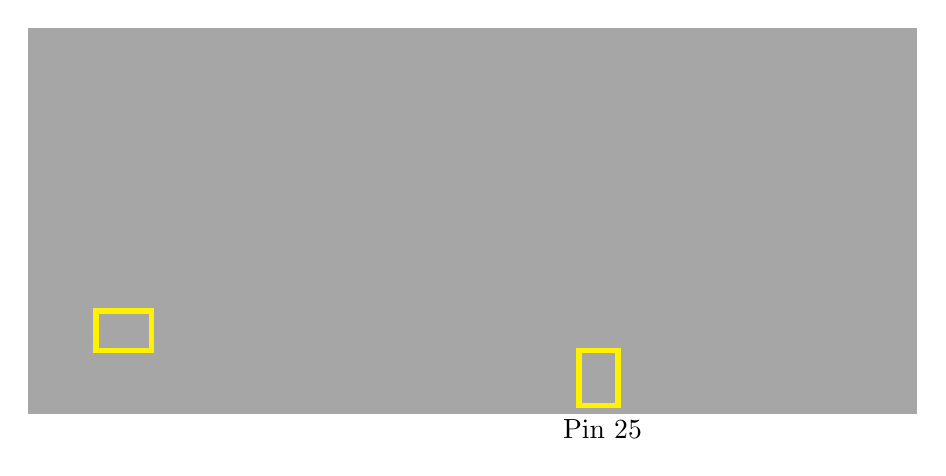
\begin{tikzpicture}
    %\node at (0,0) (Board) {\includegraphics{Arduino/Nano33BLE/Nano33BLESense}};
    
    \ArduinoNanoTikz;

    \fill[gray, opacity=0.7] (-11.2,-0.2) rectangle (0.1,4.7);
    
    \coordinate (A) at (-10.33,0.6);
    \coordinate (B) at (-9.63,1.1);    

    \coordinate (C) at (-4.2,0.6);
    \coordinate (D) at (-3.7,-0.1);    
    
    
    \begin{scope}
      \clip (A) rectangle (B);
      
      \ArduinoNanoTikz

      %\node at (0,0) (Board) {\includegraphics{Arduino/Nano33BLE/Nano33BLESense}};

    \end{scope}


    \draw[yellow,line width=2pt] (A)  rectangle (B);
    \draw[yellow,line width=2pt] (C)  rectangle (D);
    
    \node (P25) at (-3.9, -0.4) {Pin 25};
  \end{tikzpicture}    

  \captionof{figure}{Arduino Nano 33 BLE Sense's Power LED with Pin 25}  
\end{center}


    

\section{Specification}


\subsection{Pin Assignment}

The power LED is a green \ac{led} and connected to pin 25.\index{Pin!Pin 25} The brightness can be controlled via \ac{pwm}. \cite{Arduino:2023a,Arduino:2023}

\begin{description}
    \item [Power LED:] \PYTHON{LED\_PWR =  25u}
\end{description}

Power LED is active-high and connected to pin 25.

The power LED can also be controlled programmatically by setting the pin to \PYTHON{HIGH} or \PYTHON{LOW}. 


The pin must be defined as an output in the function \PYTHON{setup} by setting \PYTHON{pinMode (LED\_PWR, OUTPUT)}, otherwise the \ac{led} cannot be switched on.

\medskip 


%Let's say we have a 200 Ohm resistor. With 5V from the Arduino and 2V across the LED, that leaves 3V across the resistor. Using [u]Ohm's Law[/u] 4, we can calculate the current. 3V/200 Ohms = 0.015 Amps (15mA). The same 15mA is flowing through the LED with 2V across it, so we have 30mW of power dissipated in the LED (2V x 15mA). Plus 45mW wasted in the resistor (3V x 15mA). Or if you want the total power coming out of the Arduino, 5V x 15mW = 75mW, which is the same as 30mW + 45mW.

\subsection{Power Comsumption}\label{LEDPowerComsumption}

The power comsumption has to be considered. There, the power and current in a simple circuit using a resistor and an LED has to calculated.

The led onboard works in a circuit with an 200 Ohm resistor, a 5V power source from an Arduino, and an LED with 2V across it. To find out how much power is being used by the LED and the resistor, the current must be calculated in the first step. Using Ohm's Law $V = I \cdot R$ we can find the current flowing through the resistor. Since 3V is across the resistor, we can plug in the values:

\medskip

$$\frac{3\hbox{V}}{200 \Omega} = 0.015 \hbox{A} = 15\hbox{mA}$$

\medskip

This means that $15$mA of current is flowing through the resistor and the LED. In the next step, we calculate the power. Now that we know the current, we can calculate the power dissipated in the LED and the resistor.

\begin{itemize}
  \item For the LED: $2$V $\times$ $15$mA $= 30$mW
  \item For the resistor: $3$V $\times$ $15$mA = $45$mW
  \item Total Power:

     To find the total power coming out of the Arduino, we multiply the voltage by the current:

              $5$V $\times$ $15$mA = $75$mW
\end{itemize}

\medskip

Notice that the total power (75mW) is equal to the sum of the power dissipated in the LED (30mW) and the resistor (45mW). This makes sense, since all the power coming out of the Arduino is being used by either the LED or the resistor.


\medskip

The pin 25 can also be used otherwise. Then the \ac{led} is just switched on if the board is connected to a power source. %\Mynote{to be tested!}

%\Mynote{What happen if there is another \ac{led} at the pin? Both in use?}

%\section{Calibration}
%
%cite method

\section{Simple Code}

\subsection{Simple Code for LEDs}

Using of LEDs is a standard problem for Arduino's programmer. Therefore, a simple library is introduced here.

\medskip

In the header file \FILE{LED.h}, see code \ref{Nano:LEDHeader}, are the declaration of the functions. There are 3 functions:

\begin{enumerate}
    \item \PYTHON{LEDinit}: This funtion initializes a digital pin of the LED as an output.
    \item \PYTHON{LED}: This funtion switches the LED  on or off.
    \item \PYTHON{LEDBrightness}: This funtion sets the LED's brightness.
\end{enumerate}

{
    \captionof{code}{Header file without comments  for using a LED}\label{Nano:LEDHeader}
    \ArduinoExternal{linerange={12-17,33-34,47-48,63-64,67}}{../../Code/Nano33BLESense/LEDs/LED.h}
}

In the file \FILE{LED.cpp}, see code \ref{Nano:LEDCpp}, the functions are implemented.

{
    \captionof{code}{Code file without comments for using a LED}\label{Nano:LEDCpp}
    \ArduinoExternal{linerange={9-11,26-32,45-57,71-89}}{../../Code/Nano33BLESense/LEDs/LED.cpp}
}


\subsection{Simple Code for the Power LED}

For using the power  LED, a simple library is introduced here.

\medskip


In the header file \FILE{PowerLED.h}, see code \ref{Nano:PowerLEDHeader}, are the declaration of the variables and the  functions. A variable is connected to pin 25.\index{Pin!Pin 25} The pin 25 is defined as an output in the function \PYTHON{PowerLEDinit}. There are  2 functions:

\begin{enumerate}
    \item \PYTHON{PowerLEDinit}: This funtion initializes a the digital pin 25 of the power LED as an output.
    \item \PYTHON{PowerLED}: This funtion switches the power LED  on or off.
\end{enumerate}

{
    \captionof{code}{Header file with doxygen comments for using the Power LED}\label{Nano:PowerLEDHeader}
    \ArduinoExternal{linerange={9-14,27-28,40-42}}{../../Code/Nano33BLESense/LEDs/PowerLED.h}
}

In the file \FILE{PowerLED.cpp}, see code \ref{Nano:PowerLEDCpp}, the functions are implemented.

{
    \captionof{code}{Code file with doxygen comments for using the Power LED}\label{Nano:PowerLEDCpp}
    \ArduinoExternal{linerange={12-15,28-34,46-51}}{../../Code/Nano33BLESense/LEDs/PowerLED.cpp}
}


\subsection{Simple Code for Testing the Power LED}


In the sketch \ref{Nano:PowerLEDTest}, the power LED is tested. First, the function \PYTHON{PowerLEDinit} is called in the  function \PYTHON{setup}. In the function \PYTHON{loop}, the power LED is switched on for 1 second and switched off for 1 second so that the power LED flashes accordingly.



{
  \captionof{code}{Simple sketch to control the power LED}\label{Nano:PowerLEDTest}
  \ArduinoExternal{linerange={16-18,30-34,46-56}}{../../Code/Nano33BLESense/Test/TestLEDPower.ino}
}

\bigskip

This is just a simple example. The variable \PYTHON{LED\_PWR} is already defined, so the assignment is not necessary. The command \PYTHON{delay} should be avoided in an Arduino sketch. Instead, variables of the type \PYTHON{elapsedMillis} should be used. \cite{ArduinoLanguage:2024}

%\Mynote{Arduino Referenz \url{https://github.com/pfeerick/elapsedMillis/wiki}}




\subsection{Test all Functions}

The brightness of the power LED can be controlled. This is demonstrated in the example sketch \ref{Nano:PowerLEDTestPWM}.

Using the pulse width modulation, the brightness is gradually increased to the maximum value and then gradually reduced to 0 again.




{
    \captionof{code}{Simple sketch to check the battery state using the power LED}\label{Nano:PowerLEDTestPWM}
    \ArduinoExternal{linerange={11-18,30-34,46-60}}{../../Code/Nano33BLESense/Test/TestLEDPowerBrightness.ino}
}



\section{Simple Application}

There are different situations where it might be useful to program the power LED of the Arduino Nano. For example, you could use it to:

\begin{itemize}
    \item Indicate the status of the board, such as whether it is connected to a power source, a computer, or a sensor.
    \item  Display the battery level of the board, by changing the brightness or color of the power \ac{led}.
    \item Create a visual alarm or notification, by making the power LED blink or flash in a certain pattern.
\end{itemize}

\medskip

The next sketch is a frame for applications with a sign of life. The power LED is switched on for 1 sec and off for 29 sec. The file \FILE{SignsOfLife.h}, see \ref{Nano:SignsOfLife}, contains the declarations and the file \FILE{SignsOfLife.cpp} contains the implementations. 


{
    \captionof{code}{Simple code for signs of life}\label{Nano:SignsOfLife}
    \ArduinoExternal{linerange={11-25,43-44,56-61}}{../../Code/Nano33BLESense/LEDs/SignsOfLife.h}\label{Nano:SignsOfLifeHeader}
}


The library contains one function for initialization and one function \PYTHON{SignsOfLife}, which controls the LED.


{
    \captionof{code}{Simple code for signs of life}\label{Nano:SignsOfLife}
    \ArduinoExternal{linerange={11-13,31-52,64-84}}{../../Code/Nano33BLESense/LEDs/SignsOfLife.cpp}\label{Nano:SignsOfLifecpp}
}


\medskip


A simple application is to check the condition of the battery. The sktech \ref{Nano:PowerLEDTestBattery} demonstrates, if the voltage drops too low, the power LED flashes, see \cite{Scherer:2022} for more information.

{
    \captionof{code}{Simple sketch to check the battery state using the power LED}\label{Nano:PowerLEDTestBattery}
    \ArduinoExternal{linerange={11-18,31-35,48-88,98-105}}{../../Code/Nano33BLESense/Test/TestLEDPowerBattery.ino}
}


\section{Further Readings}

\begin{itemize}
  \item Kurniawan, Agus: \textsl{IoT Projects with Arduino Nano BLE Sense: Step-By-Step Projects for Beginners}. Apress, 2021. \cite{Kurniawan:2021b}
  \item K\"uhnel, Claus: \textsl{Arduino - Das umfassende Handbuch}. Rheinwerk Verlag GmbH, 2024. \cite{Kuehnel:2024}
  \item Smythe, Richard J.: \textsl{Advanced Arduino Techniques in Science - Refine Your Skills and Projects with PCs or Python-Tkinter}. Apress, 2021. \cite{Smythe:2021}
  \item Smythe, Richard J.: \textsl{Arduino in Science - Collecting, Displaying, and Manipulation Sensor Data}. Apress, 2021. \cite{Smythe:2021b}
\end{itemize}      


